
%%%%%%%%%%%%%%%%%%%% file cmmr12_template.tex %%%%%%%%%%%%%%%%%%%%%
%
% This is the LaTeX source for the instructions to authors using
% the LaTeX document class 'llncs.cls' for contributions to
% the Lecture Notes in Computer Sciences series.
% http://www.springer.com/lncs       Springer Heidelberg 2006/05/04
%
% It may be used as a template for your own input - copy it
% to a new file with a new name and use it as the basis
% for your article.
%
% NB: the document class 'llncs' has its own and detailed documentation, see
% ftp://ftp.springer.de/data/pubftp/pub/tex/latex/llncs/latex2e/llncsdoc.pdf
%
%%%%%%%%%%%%%%%%%%%%%%%%%%%%%%%%%%%%%%%%%%%%%%%%%%%%%%%%%%%%%%%%%%%


\documentclass[runningheads,a4paper]{llncs}

\usepackage{amssymb}
\setcounter{tocdepth}{3}
\usepackage{graphicx}
\usepackage{url}
\newcommand{\keywords}[1]{\par\addvspace\baselineskip
\noindent\keywordname\enspace\ignorespaces#1}

\pagestyle{headings}

\begin{document}

\mainmatter  % start of an individual contribution

% first the title is needed
\title{From Faust to Web Audio: Compiling Faust to JavaScript using Emscripten to make noise in the browser.}

% a short form should be given in case it is too long for the running head
\titlerunning{From Faust to Web Audio}

% the name(s) of the author(s) follow(s) next
%
% NB: Chinese authors should write their first names(s) in front of
% their surnames. This ensures that the names appear correctly in
% the running heads and the author index.
%
\author{Myles Borins \thanks{Julius O. Smith, St\'{e}phane Letz, Yann Orley, and Colin Clark}}
%
% if the names of the authors are too long for the running head, please use the format: AuthorA et al.
\authorrunning{Myles Borins}

% the affiliations are given next; don't give your e-mail address
% unless you accept that it will be published
\institute{Center For Computer Research in Music and Acoustics\\ \email{mborins@ccrma.stanford.edu}}

%
% NB: a more complex sample for affiliations and the mapping to the
% corresponding authors can be found in the file "llncs.dem"
% (search for the string "\mainmatter" where a contribution starts).
% "llncs.dem" accompanies the document class "llncs.cls".
%


\maketitle


\begin{abstract}
% The abstract should summarize the contents of the paper and should
% contain at least 70 and at most 150 words. It should be written using the
% \emph{abstract} environment.
The Web Audio API is a platform for doing audio synthesis in the browser.  Currently it has a number of natively compiled audio nodes capable of doing advanced synthesis.  One of the available nodes the ``JavaScriptNode" allows individuals to create their own custom unit generators in pure JavaScript. While a number of people have been writing custom nodes, they are rewriting code that has been perfected multiple times in various languages. The Faust project, developed at Grame CNCM, offers a unique solution to this problem.  Faust consists of both a language and a compiler, allows individuals to deploy a signal processor to various architectures including Max/MSP, supercollider, and core-audio.  This paper examines a technology stack that allows for Faust to be compiled to highly optimized JavaScript unit generators that synthesize sound using the Web Audio API.  


\keywords{Faust, Flocking, WAAX, JavaScript, asm.js, Emscripten}
\end{abstract}


\section{Introduction}

The Web Audio API, released in 2011, is ``a high-level JavaScript API for processing and synthesizing audio in web applications."\footnote{\url{https://dvcs.w3.org/hg/audio/raw-file/tip/Web Audio/specification.html}}  Currently there are a number of natively compiled audio nodes within the API capable of doing various forms of synthesis and digital signal processing. One of the available nodes, the ``JavaScriptNode", allows individuals to create their own custom unit generators in pure JavaScript, extending the Web Audio API.

While the concept of making interactive sound synthesis environments in the browser is quite exciting, there are two primary factors stopping individuals from investing time into the Web Audio platform; There has not yet been enough Signal Processing related JavaScript code written yet, and some signal processing concepts prove difficult to implement efficiently in a loosely typed language with no memory management.

\section{WAAX and Flocking}

There are a number of projects that are in development abstracting over top of the Web Audio API in order to extend its capabilities, create more complicated unit generators, and allow for a more intuitive syntax.  Projects such as WAAX (Web Audio API eXtension)\footnote{\url{https://github.com/hoch/waax}} by Hongchan Choi do so while using only the natively compiled nodes in order to ensure optimum efficiency.\cite{waax}

While these projects offer a wide variety of unit generators and synthesis modules, they cannot be used to implement all cutting edge techniques.  For example the delay node interface does not offer a tap in or tap out function, making wave guide models impossible to implement.\footnote{\url{https://dvcs.w3.org/hg/audio/raw-file/tip/Web Audio/specification.html#DelayNode-section}}

The Flocking audio synthesis toolkit\footnote{\url{http://flockingjs.org/}} by Colin Clark offers a unique declarative model for doing signal processing within the browser.  Unlike WAAX, Flocking has opted to use the ``JavaScriptNode" for all unit generators giving users access to a number of signal processing algorithms that can not be achieved using only native nodes.

WAAX and Flocking offer two very different approaches to Web Audio. WAAX offers efficiency, whereas Flocking offers bleeding edge unit generators and declarative syntax.  That being said both projects suffer from the same problem, a lack of man hours.  There are only so many individuals who have the time and domain specific knowledge necessary to contribute to their development.

\section{Faust}
The Faust project offers a unique solution to this problem; rather than write code, generate it.  Faust, developed at Grame CNCM,``is a programming language that provides a purely functional approach to signal processing while offering a high level of performance." \cite{orlarey:09c}  The project is both a language and a compiler, offering the ability to write code once and deploy to many different signal processing environments.

Faust also has a community of scientists and developers who have contributed a large amount of code waiting to be compiled to other platforms.  For example Julius Smith has done a substantial amount of research using Faust to implement wave guide synthesis models\cite{Julius:waveguide} and Romain Michon has ported the entire STK to Faust.\cite{Michon:stk}

Creating an efficient compile path from Faust to the Web Audio API would allow for all of the available Faust code to immediately be able to run in the browser. Further, using the architecture compilation model that Faust is famous for we would be able to wrap the compiled Web Audio code to be compatible with all current libraries and frameworks such as WAAX and Flocking.

\section{Current Web Audio Implementation}

Currently there is an implementation done by St\'{e}phane Letz to compile Faust to Web Audio directly from the Faust Intermediate Representation\footnote{\url{http://faust.grame.fr/index.php/7-news/73-faust-web-art}}.  This implementation currently has a number of problems.  While the implementation is elegant, any algorithms relying on integer arithmetic are currently broken due to JavaScript representing all variables as 32-bit floating point at a lower level.

\section{And now for something completely different}

\subsection{asm.js}

A potential solution to the problem of lower level variable represetation is asm.js.  Asm.js ``is a strict subset of JavaScript that can be used as a low-level, efficient target language for compilers. The asm.js language provides an abstraction similar to the C/C++ virtual machine: a large binary heap with efficient loads and stores, integer and floating-point arithmetic, first-order function definitions, and function pointers."\cite{asm-js}

\subsection{Emscripten}

As mentioned above asm.js is designed to be a target language for compilers.  While it would be possible to work with the current implementation of Faust to Web Audio to utilize asm.js in order to get specific types there are a number of project that currently exist that have development teams working to make the process as efficient as possible.

Emscripten is a project started by Alon Zakai from Mozilla that compiles LLVM(Low Level Virtual Machine) assembler to JavaScript, specifcally asm.js.\cite{Emscripten} Currently Faust is able to compile to a barebones C++ file using the minimal.cpp architecture file, the resulting file can painlessly be compiled to asm.js with Emscripten.  The upstream Faust2 branch can compile Faust to LLVM byte-code which could potentially be another compilation path.

\section{Making Noise}

A first approach to automating the compilation process from Faust to Web Audio involves manually implementing each step. The Faust code needs to be compiled to C++ and have the resulting dsp class wrapped in order to allow internal data and member function to be accessed once compiled to JavaScript.  The resulting C++ file then needs to be compiled by Emscripten to asm.js.  The asm.js needs to once again be wrapped in order to recreate the original C++ object as a JavaScript object.  These functions then need to be hooked into the Web Audio API.

As an initial proof of concept it was attempted to compile the example noise.dsp that comes shipped with Faust to JavaScript by way of Emscripten. Noise was a prime candidate for these initial tests due to the integer specific calculations used in its algorithm.

The below sections will describe the process used to manually implement noise in the browser starting from a faust dsp file, and ending with a working Web Audio API JavaScript Object.

\subsection{Faust}

The noise unit generator starts as a Faust dsp file.

\begin{verbatim}
    random  = +(12345)~*(1103515245);
    noise   = random/2147483647.0;
    process = noise * 0.5;
\end{verbatim}

In order to compile to C++ in a manner that will be compatible with Emscripten we must use the follow command.

\begin{verbatim}
    faust -a minimal.cpp -i -uim -cn Noise  dsp/noise.dsp \
      -o cpp/faust-noise.cpp
\end{verbatim}

The resulting file must then be wrapped in a way to allow its functions to be accessed once compiled to JavaScipt. The source for this wrapper can be found within the code repository on GitHub, a link for which is found at the end of this paper.  The wrapper creates five functions, a constructor, a destructor, a function to get the number of inputs / outputs, and a compute function. These functions are all placed in an `extern' in order to avoid name space obfuscation.
\subsection{Emscripten \& asm.js}

Once the wrapper has been concatenated with the Faust compiled C++ it can then be compiled by Emscripten to asm.js.  This is done with the following command 

\begin{verbatim}
    emcc cpp/faust-noise.cpp -o js/faust-noise-temp.js \
      -s EXPORTED_FUNCTIONS="['_NOISE_constructor', \ 
      '_NOISE_destructor', '_NOISE_compute', \
      '_NOISE_getNumInputs', '_NOISE_getNumOutputs']"
\end{verbatim}

Note the exported functions, which are referencing the five wrapper functions mentioned in the previous step.  This is required to stop Emscripten from obfuscating the names of the functions when certain optimization flags are thrown during compilation

\subsection{Web Audio Api}

Once the asm.js code has been compiled a JavaScript wrapper is used break out the functionality of the code into JavaScript functions.  As well, the correct context for generating audio in the browser needs to be set up within the Web Audio API, connecting the generated data from the Faust generated functions to the correct Web Audio API functions in order to generate sound. Again this wrapper can be found in the source repository on GitHub


% \section{Automation}
% 
% All the above steps should be able to be automated, if time permits this section will examine how an architecture file can be written in order to compile any faust dsp file to the Web Audio API and Flocking.

\section{Results}

Using the above methods a Faust compiled WebAudio noise unit generator was successfully created.  The result can be found at:

     \url{https://ccrma.stanford.edu/~mborins/420b/demo/}
     
\section{Limitations}

There were a few limitations that were found with the current compilation method.  First, we can currently only use Faust code that requires no input and only a single output channel.  This is due to the fact that managing memory in C++ while maintaing persistence when compiled to JavaScript can be tricky. Specifically because Faust represents inputs and outputs as a float **.  More research needs to be done in to JavaScript pointer arithmetic before this problem will be able to be solved.

A second problem is that Faust relies on UI as a control interface to make any changes to the state of a unit generator.  As such current code that relies on this would need to be modified prior to working with the current tool chain.  Rather than requiring individuals to manually augment all previously written code, a solution needs to be found to allow current UI elements to be interpreted in a way that changes can be made through events in JavaScript.

Finally the current compilation path is hard coded, there is no way to compile other unit generators without going through the entire process again from scratch.  A solution to this problem will most likely be simple, but implementing it without polluting the global name space of JavaScript could prove challenging.

\section{Looking Forward}

While the above mentioned limitations do needs to be worked on, benchmarks should be performed on the currently compiling code to ensure that this compilation method is in fact a good direction.  Colin Clark has offered to implement some benchmark tests against his Flocking library as well as a number of other WebAudio based implementations if he can be provided a working version of freeverb.  Due to this generous offer, creating a working freeverb will most likely be the next logical step in for this research.

As well, St\'{e}phane Letz and Yann Orley have expressed a desire to approach this problem using their original method of going directly from the Faust Intermediate Representation to JavaScript.  This would avoid moving from a functional language to an object oriented language back to a function language, which has proven somewhat inelegant.  It may prove appropriate once the Emscripten method can be benchmarked to put time in to developing this more direct compilation path so that the results from the two methods can be compared.

\section{Conclusion}

The results of this research have shown that it is indeed possible to get compiled Faust code running properly in the browser.  This is very exciting, as if the benchmarks are encouraging we will be able to use the resulting code to greatly expand the ecosystem for digital signal processing in the browser.

One of the most exciting parts of the results are that if this process can be perfected we will continue to see improvements in efficiency as the various technologies we are relying on continue to improve.  As JavaScript becomes more efficient, so does the compiled code.  As WebAudio becomes more stable, so does the compiled code. As asm.js optimizations improve in the browser, we get the optimizations for free.  Simply put, even if the resulting benchmarks prove to not be competitive with current hand written JavaScript, it will only get better with time while requiring minimal time maintaing the project.

\section{Code Repository}

The entire source code can be found online on GitHub at:
\\
\url{https://github.com/TheAlphaNerd/faust2webaudio}

\begin{thebibliography}{1}
	
    % \bibitem{orlarey:09c}
    % Y.~Orlarey, D.~Fober, and S.~Letz.
    %      \textsl{New Computational Paradigms for Computer Music},
    % \newblock 2009.

    \bibitem{waax}
    H.~Choi, J.Berger., ``WAAX: Web Audio API eXtension"
    \emph{Proceedings of the Thirteenth New Interfaces for Musical Expression Conference}, 2013.
    
	
    \bibitem{orlarey:09c} Y.~Orlarey, D.~Fober, and S.~Letz., ``FAUST : an Efficient Functional Approach to DSP Programming,"
    \emph{New Computational Paradigms for Computer Music}, pp. 65-96, Editions DELATOUR FRANCE, 2009.
    
    \bibitem{Julius:waveguide} J. Smith, J. Kuroda, J. Perng, K. V. Heusen, and J. Abel, ``Efficient computational modeling of piano strings for real-time synthesis using mass-spring chains, coupled finite differences, and digital waveguide sections"
    \emph{Acoustical Society of America, Program of the 2nd Pan-American/Iberian Meeting on Acoustics (abstract and presentation)}, Cancun, Mexico, Nov. 15–19, 2010, invited presentation. Presentation overheads: https://ccrma.stanford.edu/~jos/pdf/ASA-2010-jos.pdf

    \bibitem{Michon:stk} R. Michon and J. O. Smith, ``Faust-STK: A set of linear and nonlinear physical models for the Faust programming language", in
    \emph{Proceedings of the 14th International Conference on Digital Audio Effects (DAFx-11),} Paris, France, September 19–23, 2011

    \bibitem{Emscripten}A. Zakai. ``Emscripten: an llvm-to-javascript compiler.''
    \emph{Proceedings of the ACM international conference companion on Object oriented programming systems languages and applications companion.} ACM, 2011.
	\bibitem{asm-js}
	\textsl{asm.js - frequently asked questions.}
    \newblock \url{http://asmjs.org/faq.html.}
    
    
	
\end{thebibliography}

% \section{Paper Preparation}
% 
% Springer provides you with a complete integrated \LaTeX{} document class
% (\texttt{llncs.cls}) for multi-author books such as those in the LNCS
% series. Papers not complying with the LNCS style will be reformatted.
% This can lead to an increase in the overall number of pages. We would
% therefore urge you not to squash your paper.
% 
% Please always cancel any superfluous definitions that are
% not actually used in your text. If you do not, these may conflict with
% the definitions of the macro package, causing changes in the structure
% of the text and leading to numerous mistakes in the proofs.
% 
% If you wonder what \LaTeX{} is and where it can be obtained, see the
% ``\textit{LaTeX project site}'' (\url{http://www.latex-project.org})
% and especially the webpage ``\textit{How to get it}''
% (\url{http://www.latex-project.org/ftp.html}) respectively.
% 
% When you use \LaTeX\ together with our document class file,
% \texttt{llncs.cls},
% your text is typeset automatically in Computer Modern Roman (CM) fonts.
% Please do
% \emph{not} change the preset fonts. If you have to use fonts other
% than the preset fonts, kindly submit these with your files.
% 
% Please use the commands \verb+\label+ and \verb+\ref+ for
% cross-references and the commands \verb+\bibitem+ and \verb+\cite+ for
% references to the bibliography, to enable us to create hyperlinks at
% these places.
% 
% For preparing your figures electronically and integrating them into
% your source file we recommend using the standard \LaTeX{} \verb+graphics+ or
% \verb+graphicx+ package. These provide the \verb+\includegraphics+ command.
% In general, please refrain from using the \verb+\special+ command.
% 
% Remember to submit any further style files and
% fonts you have used together with your source files.
% 
% \subsubsection{Headings.}
% 
% Headings should be capitalized
% (i.e., nouns, verbs, and all other words
% except articles, prepositions, and conjunctions should be set with an
% initial capital) and should,
% with the exception of the title, be aligned to the left.
% Words joined by a hyphen are subject to a special rule. If the first
% word can stand alone, the second word should be capitalized.
% 
% Here are some examples of headings: ``Criteria to Disprove
% Context-Freeness of Collage Language", ``On Correcting the Intrusion of
% Tracing Non-deterministic Programs by Software", ``A User-Friendly and
% Extendable Data Distribution System", ``Multi-flip Networks:
% Parallelizing GenSAT", ``Self-determinations of Man".
% 
% \subsubsection{Lemmas, Propositions, and Theorems.}
% 
% The numbers accorded to lemmas, propositions, and theorems, etc. should
% appear in consecutive order, starting with Lemma 1, and not, for
% example, with Lemma 11.
% 
% \subsection{Figures}
% 
% For \LaTeX\ users, we recommend using the \emph{graphics} or \emph{graphicx}
% package and the \verb+\includegraphics+ command.
% 
% Please check that the lines in line drawings are not
% interrupted and are of a constant width. Grids and details within the
% figures must be clearly legible and may not be written one on top of
% the other. Line drawings should have a resolution of at least 800 dpi
% (preferably 1200 dpi). The lettering in figures should have a height of
% 2~mm (10-point type). Figures should be numbered and should have a
% caption which should always be positioned \emph{under} the figures, in
% contrast to the caption belonging to a table, which should always appear
% \emph{above} the table; this is simply achieved as matter of sequence in
% your source.
% 
% Please center the figures or your tabular material by using the \verb+\centering+
% declaration. Short captions are centered by default between the margins
% and typeset in 9-point type (Fig.~\ref{fig:example} shows an example).
% The distance between text and figure is preset to be about 8~mm, the
% distance between figure and caption about 6~mm.
% 
% To ensure that the reproduction of your illustrations is of a reasonable
% quality, we advise against the use of shading. The contrast should be as
% pronounced as possible.
% 
% If screenshots are necessary, please make sure that you are happy with
% the print quality before you send the files.
% \begin{figure}
% \centering
% 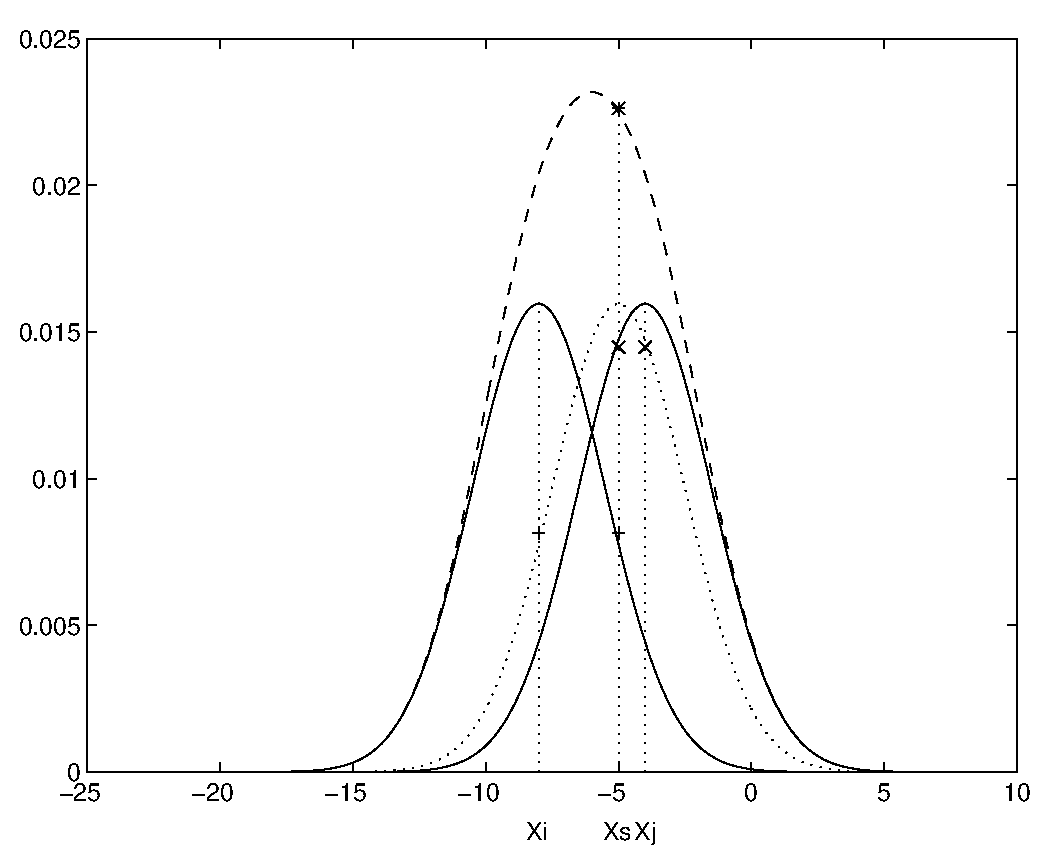
\includegraphics[height=6.2cm]{eijkel2}
% \caption{One kernel at $x_s$ (\emph{dotted kernel}) or two kernels at
% $x_i$ and $x_j$ (\textit{left and right}) lead to the same summed estimate
% at $x_s$. This shows a figure consisting of different types of
% lines. Elements of the figure described in the caption should be set in
% italics, in parentheses, as shown in this sample caption.}
% \label{fig:example}
% \end{figure}
% 
% Please define figures (and tables) as floating objects. Please avoid
% using optional location parameters like ``\verb+[h]+" for ``here".
% 
% \paragraph{Remark 1.}
% 
% In the printed volumes, illustrations are generally black and white
% (halftones), and only in exceptional cases, and if the author is
% prepared to cover the extra cost for color reproduction, are colored
% pictures accepted. Colored pictures are welcome in the electronic
% version free of charge. If you send colored figures that are to be
% printed in black and white, please make sure that they really are
% legible in black and white. Some colors as well as the contrast of
% converted colors show up very poorly when printed in black and white.
% 
% \subsection{Formulas}
% 
% Displayed equations or formulas are centered and set on a separate
% line (with an extra line or halfline space above and below). Displayed
% expressions should be numbered for reference. The numbers should be
% consecutive within each section or within the contribution,
% with numbers enclosed in parentheses and set on the right margin --
% which is the default if you use the \emph{equation} environment, e.g.,
% \begin{equation}
%   \psi (u) = \int_{o}^{T} \left[\frac{1}{2}
%   \left(\Lambda_{o}^{-1} u,u\right) + N^{\ast} (-u)\right] dt \;  .
% \end{equation}
% 
% Equations should be punctuated in the same way as ordinary
% text but with a small space before the end punctuation mark.
% 
% \subsection{Footnotes}
% 
% The superscript numeral used to refer to a footnote appears in the text
% either directly after the word to be discussed or -- in relation to a
% phrase or a sentence -- following the punctuation sign (comma,
% semicolon, or period). Footnotes should appear at the bottom of
% the
% normal text area, with a line of about 2~cm set
% immediately above them.\footnote{The footnote numeral is set flush left
% and the text follows with the usual word spacing.}
% 
% \subsection{Program Code}
% 
% Program listings or program commands in the text are normally set in
% typewriter font, e.g., CMTT10 or Courier.
% 
% \medskip
% 
% \noindent
% {\it Example of a Computer Program}
% \begin{verbatim}
% program Inflation (Output)
%   {Assuming annual inflation rates of 7%, 8%, and 10%,...
%    years};
%    const
%      MaxYears = 10;
%    var
%      Year: 0..MaxYears;
%      Factor1, Factor2, Factor3: Real;
%    begin
%      Year := 0;
%      Factor1 := 1.0; Factor2 := 1.0; Factor3 := 1.0;
%      WriteLn('Year  7% 8% 10%'); WriteLn;
%      repeat
%        Year := Year + 1;
%        Factor1 := Factor1 * 1.07;
%        Factor2 := Factor2 * 1.08;
%        Factor3 := Factor3 * 1.10;
%        WriteLn(Year:5,Factor1:7:3,Factor2:7:3,Factor3:7:3)
%      until Year = MaxYears
% end.
% \end{verbatim}
% %
% \noindent
% {\small (Example from Jensen K., Wirth N. (1991) Pascal user manual and
% report. Springer, New York)}
% 
% \subsection{Citations}
% 
% For citations in the text please use
% square brackets and consecutive numbers: \cite{jour}, \cite{lncschap},
% \cite{proceeding1} -- provided automatically
% by \LaTeX 's \verb|\cite| \dots\verb|\bibitem| mechanism.
% 
% \subsection{Page Numbering and Running Heads}
% 
% There is no need to include page numbers. If your paper title is too
% long to serve as a running head, it will be shortened. Your suggestion
% as to how to shorten it would be most welcome.
% 
% 
% \section{BibTeX Entries}
% 
% The correct BibTeX entries for the Lecture Notes in Computer Science
% volumes can be found at the following Website shortly after the
% publication of the book:
% \url{http://www.informatik.uni-trier.de/~ley/db/journals/lncs.html}
% 
% \subsubsection*{Acknowledgments.} The heading should be treated as a
% subsubsection heading and should not be assigned a number.
% 
% \section{The References Section}\label{references}
% 
% In order to permit cross referencing within LNCS-Online, and eventually
% between different publishers and their online databases, LNCS will,
% from now on, be standardizing the format of the references. This new
% feature will increase the visibility of publications and facilitate
% academic research considerably. Please base your references on the
% examples below. References that don't adhere to this style will be
% reformatted by Springer. You should therefore check your references
% thoroughly when you receive the final pdf of your paper.
% The reference section must be complete. You may not omit references.
% Instructions as to where to find a fuller version of the references are
% not permissible.
% 
% We only accept references written using the latin alphabet. If the title
% of the book you are referring to is in Russian or Chinese, then please write
% (in Russian) or (in Chinese) at the end of the transcript or translation
% of the title.
% 
% The following section shows a sample reference list with entries for
% journal articles \cite{jour}, an LNCS chapter \cite{lncschap}, a book
% \cite{book}, proceedings without editors \cite{proceeding1} and
% \cite{proceeding2}, as well as a URL \cite{url}.
% Please note that proceedings published in LNCS are not cited with their
% full titles, but with their acronyms!
% 
% \begin{thebibliography}{4}
% 
% \bibitem{jour} Smith, T.F., Waterman, M.S.: Identification of Common Molecular
% Subsequences. J. Mol. Biol. 147, 195--197 (1981)
% 
% \bibitem{lncschap} May, P., Ehrlich, H.C., Steinke, T.: ZIB Structure Prediction Pipeline:
% Composing a Complex Biological Workflow through Web Services. In: Nagel,
% W.E., Walter, W.V., Lehner, W. (eds.) Euro-Par 2006. LNCS, vol. 4128,
% pp. 1148--1158. Springer, Heidelberg (2006)
% 
% \bibitem{book} Foster, I., Kesselman, C.: The Grid: Blueprint for a New Computing
% Infrastructure. Morgan Kaufmann, San Francisco (1999)
% 
% \bibitem{proceeding1} Czajkowski, K., Fitzgerald, S., Foster, I., Kesselman, C.: Grid
% Information Services for Distributed Resource Sharing. In: 10th IEEE
% International Symposium on High Performance Distributed Computing, pp.
% 181--184. IEEE Press, New York (2001)
% 
% \bibitem{proceeding2} Foster, I., Kesselman, C., Nick, J., Tuecke, S.: The Physiology of the
% Grid: an Open Grid Services Architecture for Distributed Systems
% Integration. Technical report, Global Grid Forum (2002)
% 
% \bibitem{url} National Center for Biotechnology Information, \url{http://www.ncbi.nlm.nih.gov}
% 
% \end{thebibliography}



\end{document}
